\label{chap:machine_learning}

In questa tesi considereremo il Machine Learning come il processo che consente
la creazione di modelli in grado di apprendere autonomamente dai dati. Un
modello è costituito da un insieme di parametri e una struttura che elabora i
dati di input per produrre un output. I parametri vengono appresi durante la
fase di addestramento, in cui il modello esamina vari esempi e regola i propri
parametri di conseguenza. Gli iperparametri, d'altra parte, sono valori
definiti dall'utente prima dell'inizio dell'addestramento che influenzano la
struttura del modello e il suo comportamento durante l'addestramento.

Prima di esplorare i modelli specifici, ci concentreremo sul processo di
creazione dei modelli di Machine Learning, e vedremo come l'automatizzazione
di questo processo, attraverso l'impiego di una \textbf{pipeline}, possa
ottimizzarne l'efficienza e l'efficacia.

Il processo di creazione di un modello di Machine Learning si compone di vari
passaggi: l'estrazione dei dati, la loro preparazione e l'addestramento del
modello. Una pipeline collega questi passaggi in sequenza,
incapsulandoli in un'entità che, dall'esterno, può essere utilizzata come se
fosse il modello stesso. Questa pipeline può essere rappresentata come un
Grafo Aciclico Diretto (DAG), dove i dati fluiscono in una sola direzione,
evitando cicli, e dove ogni nodo in questo grafo rappresenta una fase distinta
del processo (vedi figura~\ref{fig:ml_pipeline_dag}).

\begin{figure}[!ht]
    \centering
    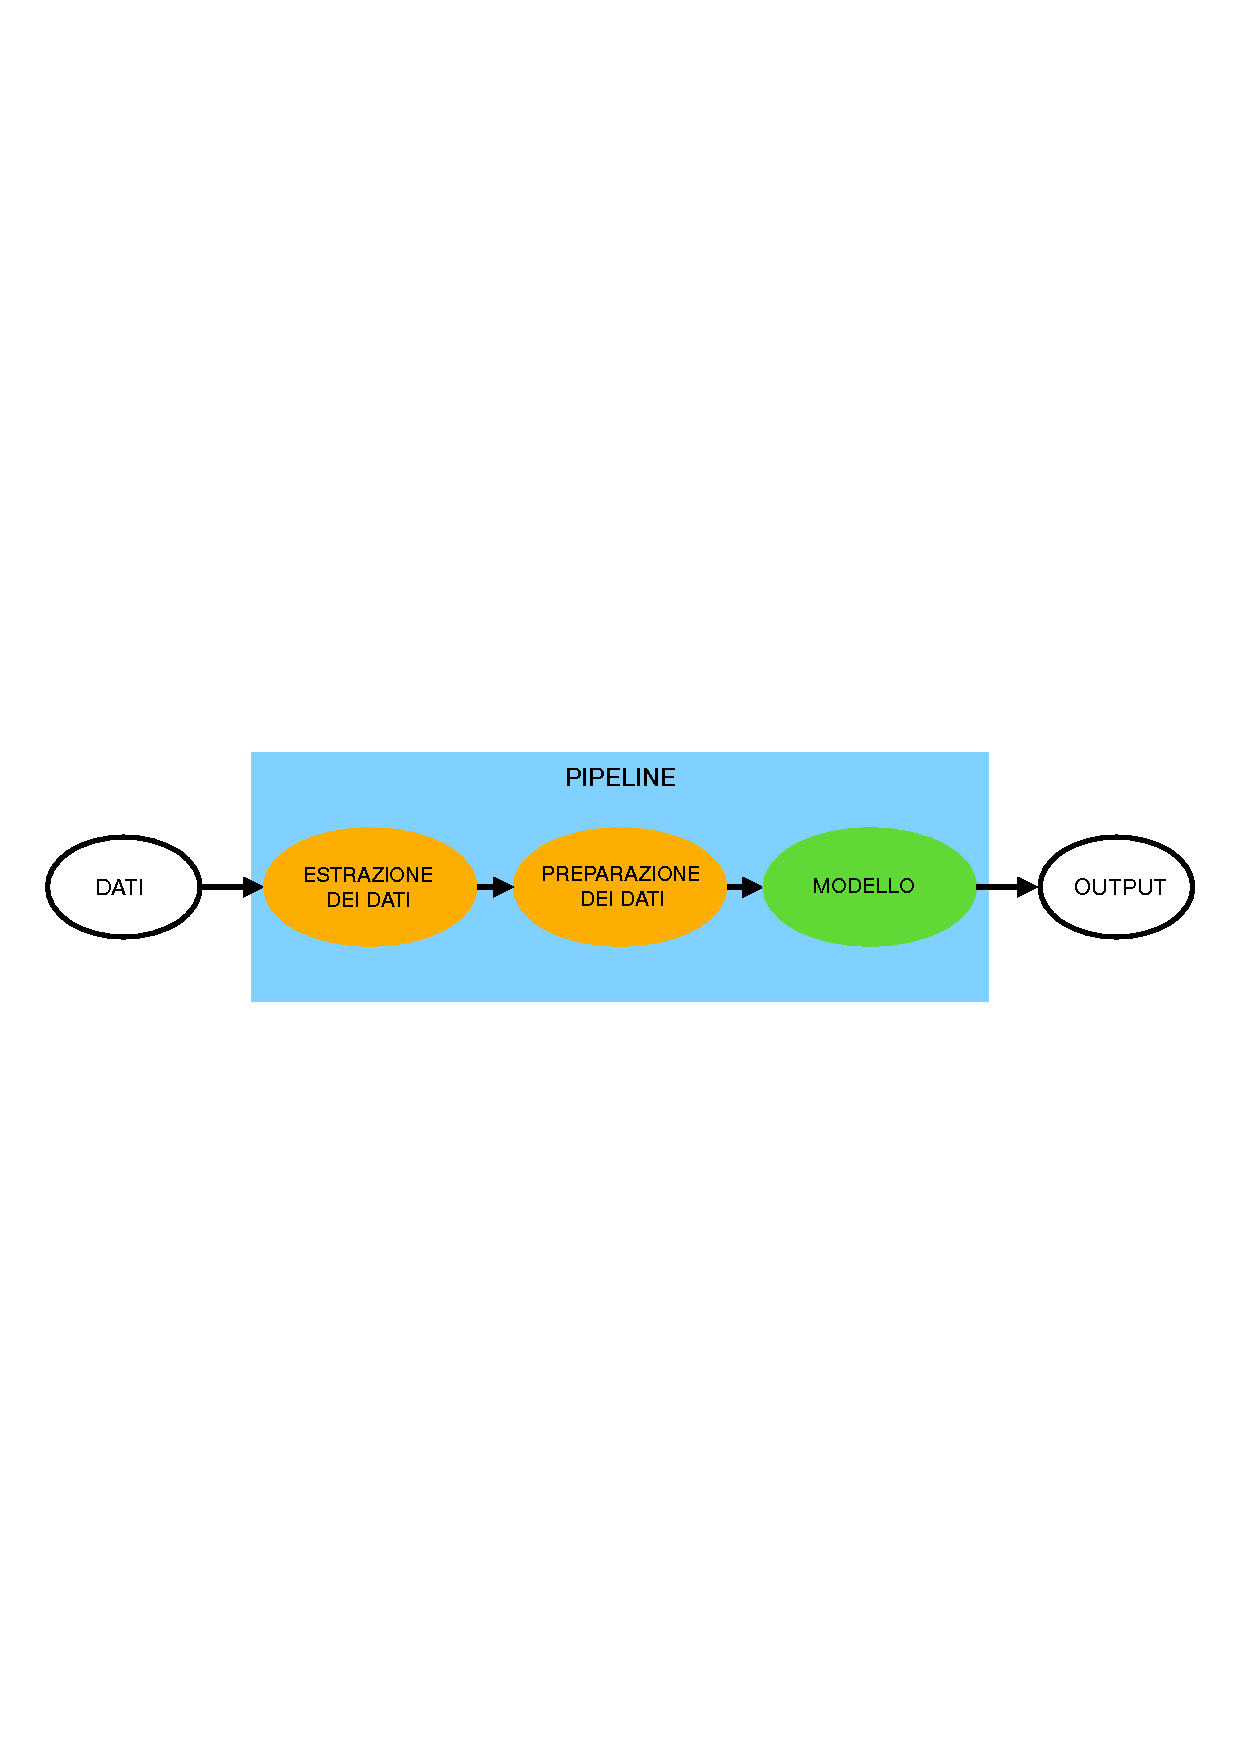
\includegraphics[trim=0 12.5cm 0 12.5cm, clip, width=\linewidth]{pipeline}
    \caption{Rappresentazione di una pipeline di Machine Learning come un
    grafo orientato senza cicli}
    \label{fig:ml_pipeline_dag}
\end{figure}

L'uso di una pipeline nel Machine Learning ci permette di ottenere i seguenti
vantaggi:
\begin{itemize}
    \item[\textit{Efficacia}] \textbf{Estensione della ricerca degli iperparametri ad altri
        componenti}: Mentre l'individuazione dei parametri migliori per un
        modello avviene in modo automatico durante l'addestramento, la ricerca
        degli iperparametri migliori richiede sperimentazioni multiple,
        testando diversi valori e valutando i risultati del modello secondo
        metriche prestabilite. Dato che esternamente una pipeline funziona
        esattamente come un modello, è possibile estendere la ricerca degli
        iperparametri migliori a componenti non direttamente correlati al
        modello stesso, come quelle legate all'estrazione e alla preparazione
        dei dati. Poiché anche la ricerca degli iperparametri è
        automatizzabile, è possibile testare automaticamente diverse tecniche
        di preparazione dei dati, semplicemente integrando il componente alla
        pipeline.
    \item [\textit{Efficienza}]\textbf{Sperimentazione rapida}: L'organizzazione di tutti i
        passaggi in una pipeline può accelerare notevolmente la
        sperimentazione. Questo è particolarmente utile quando si prevede di
        testare vari iperparametri o di utilizzare differenti sottoinsiemi di
        dati. Infatti, incapsulando le operazioni delle diverse componenti in
        un unico elemento che le esegue sequenzialmente, si evita di ripetere
        le stesse operazioni più volte, risultando in un risparmio di tempo
        significativo.
\end{itemize}

Nelle sezioni seguenti, descriveremo come sono stati affrontati i vari
passaggi nella creazione di un modello di Machine Learning per
l'identificazione dei job zombie e come si è cercato di integrare ciascun
componente alla pipeline.

\section{Estrazione dei dati}

L'estrazione di un dataset viene fatta tramite una query SQL che interroga le
tabelle \texttt{hj} e \texttt{htjob}, selezionando i dati rilevanti.
Ricordando che:
\begin{itemize}
    \item La tabella \texttt{hj} contiene lo stato dei job, rappresentato da
        serie storiche di misurazioni (come \texttt{runtime}, \texttt{ram},
        \texttt{swap}, \texttt{disk}, ecc.),
        durante la loro esecuzione.
    \item La tabella \texttt{htjob} fornisce informazioni sull'esito dei job,
        indicando se sono falliti o meno.
\end{itemize}

% job

%jobid e idx sono creati dal Submit Node al "concepimento" del job (es.
%'sn-01', 'ce03-htc', ...). I S.N. sono indipendenti tra loro per cui in linea
%di principio possono esistere due job diversi con (jobid,idx) uguale (in tal
%caso vengono da S.N. diversi)

% fail

%Ci sono due momenti diversi: il batch system puo' terminare LUI un job anche
%se non ha alcun problema (per una serie di ragioni) e quella info e' in
%jobstatus, Poi c'e' lo exitstatus dell'eseguibile vero e proprio: di questo
%sappiamo che se e' 0 allora e' ok, se e' != 0 e' uscito con errore (quale sia
%lo sa il suo owner).

La query esegue le seguenti operazioni:
\begin{itemize}
    \item Seleziona i job che hanno iniziato e finito la loro esecuzione nel
        periodo temporale specificato.
    \item Esegue un JOIN delle tabelle utilizzando l'identificativo univoco di
        ciascun job (\textit{jobid.idx\_submitnode}) e il timestamp. Questo
        timestamp sfrutta l'indice presente nella tabella
        \texttt{hj} per gestire in maniera efficiente le grandi dimensioni di
        questa tabella\footnote{La logica dietro questo consiste
            nel selezionare un job da \texttt{htjob} e successivamente
            cercarlo in \texttt{hj} limitando la ricerca ai record che
            rientrano nel periodo in cui \texttt{hj.ts} è compreso tra
            \texttt{htjob.starttimeepoch} e \texttt{htjob.eventtimeepoch}.
            Questo permette di restringere notevolmente la ricerca nella
            tabella \texttt{hj} per ogni job selezionato da \texttt{htjob} ed
        evitare di scansionare l'intera tabella.}. Poiché la tabella \texttt{hj} contiene più record per
        ogni job, la query li raggruppa per job. In seguito, mediante l'uso
        dell'operatore \verb|ARRAY_AGG|, le serie storiche vengono trasformate
        in liste di valori.
    \item Filtra i job con un tempo di esecuzione superiore a un'ora
        (\verb|runtime > 3600|), in quanto i job più brevi sono considerati
        irrilevanti per lo scopo dello studio.
\end{itemize}

Il risultato di questa query è un dataset come mostrato nella
figura~\ref{fig:dataset_from_join_hj_htjob}, dove ogni riga rappresenta un job
e le colonne includono: 

\begin{itemize}
    \item \texttt{job}: identificativo univoco per ogni job.
    \item \texttt{queue}: gruppo di appartenenza dell'utente che ha sottomesso
        il job.
    \item \texttt{fail}: una variabile booleana che indica se il job è fallito.
    \item \texttt{mint} e \texttt{maxt}: il tempo minimo e massimo di
        esecuzione del job.
    \item \texttt{t}, \texttt{ram}, \texttt{swap}, \texttt{disk}: liste di
        valori che rappresentano le serie storiche di misurazioni.
\end{itemize}

\begin{figure}[!ht]
    \centering
    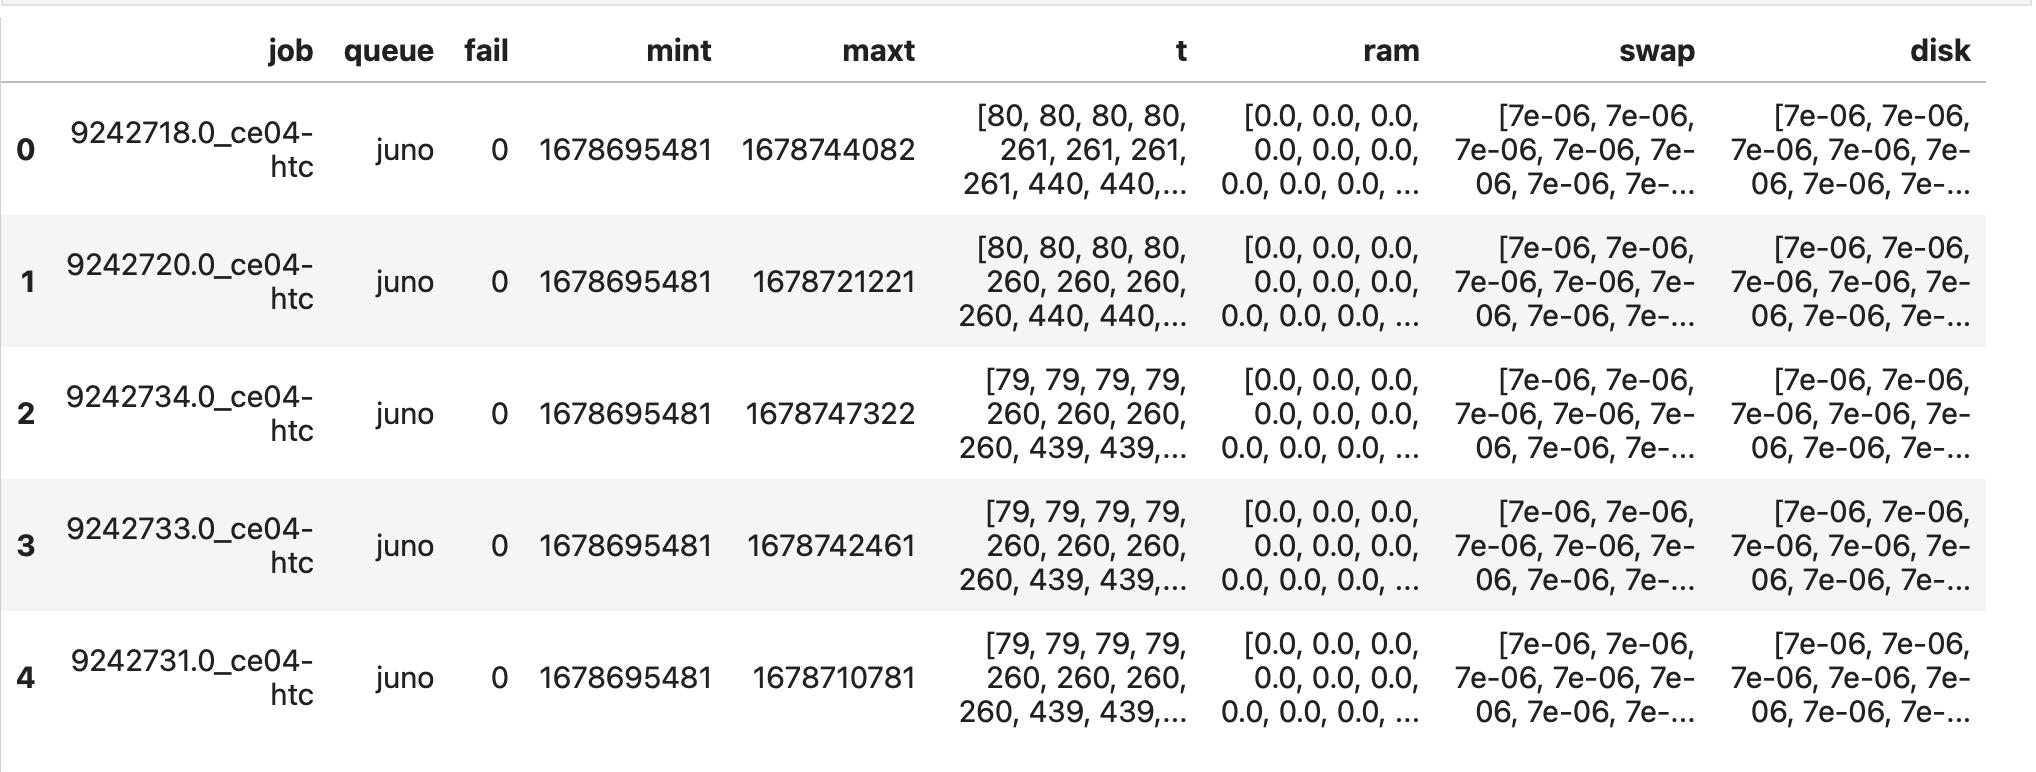
\includegraphics[width=0.95\textwidth]{dataset}
    \caption{Le prime cinque righe del dataset}
    \label{fig:dataset_from_join_hj_htjob}
\end{figure}

Tuttavia, il dataset estratto non è ancora pronto per l'addestramento del
modello e necessita di ulteriori trasformazioni da parte del componente
successivo. Questo passaggio non è stata integrato nella pipeline, in quanto,
nell'ambiente operativo reale, si prevede che questa lavori direttamente con i
dati forniti da HTCondor, eliminando così la necessità di estrarre dati da un
database SQL.

\section{Preparazione dei dati}

La preparazione dei dati è essenziale nel Machine Learning. Prima di tutto, è
necessario convertire i dati in numeri, dato che gli algoritmi di Machine
Learning lavorano esclusivamente con dati in tale forma. Inoltre, la qualità e
la quantità dei dati sono determinanti per l'efficacia del modello. Se i dati
disponibili sono insufficienti o di bassa qualità, i risultati saranno
scadenti a prescindere dalla complessità del modello utilizzato. Tipicamente,
maggiore è la complessità di un modello, tanto più esso richiederà una grande
quantità di dati di alta qualità.

Per realizzare ciò, è stata creata una classe denominata
\texttt{Preprocessor}, che riceve in input un dataset e restituisce in output
un dataset modificato, eseguendo una serie di operazioni intermedie. Queste
operazioni possono essere ricondotte a tre categorie: l'aggiunta, la rimozione
e la trasformazione di colonne. Le operazioni effettuate sono configurabili
attraverso parametri definiti nel costruttore della classe al momento della
sua istanziazione. Quando questo componente viene inserito all'interno di una
pipeline, tali parametri fungono da iperparametri, permettendo di esplorare
diverse configurazioni per identificare quale produca i risultati migliori.

In aggiunta, questa classe è stata implementata seguendo il design pattern
Template Method, nel quale i passaggi di un algoritmo vengono divisi in metodi
separati, e successivamente invocati da un metodo denominato template (vedi
figura~\ref{fig:uml_preprocessor}). La superclasse definisce lo scheletro
dell'algoritmo, consentendo alle sottoclassi di personalizzare alcuni passaggi
sovrascrivendo alcuni metodi. In questo modo, è possibile codificare la parte
invariante dell'algoritmo una sola volta nella superclasse, lasciando alle
sottoclassi il compito di implementare i comportamenti che possono variare. In
pratica, l'uso di questo pattern in questa classe ci consente di aggiungere,
modificare e rimuovere passaggi dall'algoritmo in modo semplice ed immediato,
senza la necessità di dover intervenire sul codice della classe principale.

\begin{figure}[!ht]
   \centering
   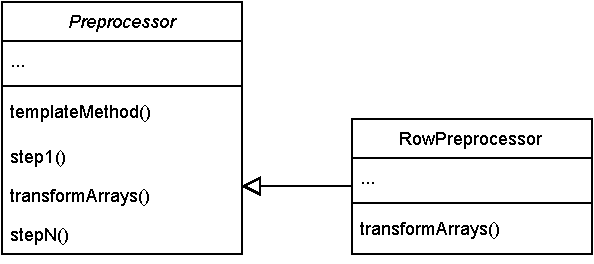
\includegraphics[width=0.5\linewidth]{preprocessor}
   \caption{Diagramma UML della classe \texttt{Preprocessor}, illustrante
   l'implementazione del design pattern Template Method}
   \label{fig:uml_preprocessor}
\end{figure}

Dopo aver delineato la struttura generale della classe \texttt{Preprocessor},
descriveremo ora le trasformazioni effettuate dal metodo
\texttt{preprocess()}, che funge da metodo template, nella preparazione dei
dati.

\subsection{Preparazione delle serie storiche}

Nella sezione~\ref{sec:job_analysis}, abbiamo identificato alcuni problemi
nelle misurazioni registrate da HTCondor relative allo stato dei job. Un
problema è la presenza di valori ripetuti all'interno delle serie storiche.
Queste serie sono attualmente rappresentate come liste di valori, che non
corrispondono al formato numerico richiesto dai modelli di Machine Learning.
Pertanto, è necessario non solo rimuovere le ripetizioni, ma anche convertire
queste serie storiche in un formato di dati strutturato.

\paragraph{Riduzione della frequenza di campionamento.} Applicando
un'operazione di convoluzione\footnote{Operazione matematica che consiste
    nell'applicare un filtro di dimensione finita lungo la sequenza di valori.
    Il filtro, di solito di piccole dimensioni, viene fatto scorrere su tutta
    la sequenza, e in ogni posizione si calcola una somma pesata tra i valori
    della sequenza e quelli del filtro. Questo processo trasforma la sequenza
    originale in una nuova attraverso la formula: $$(S\ast
K)(i)=\displaystyle\sum_{m=-d}^{d}S(m)\cdot K(i-m)$$ dove $S$ è la sequenza
originale, $K$ è il filtro e $d$ è l'intero inferiore della metà della
lunghezza del filtro.} con un passo (\textit{stride}) di 5 e un filtro di 5
elementi con valore $\frac{1}{5}$, possiamo effettuare una decimazione della
sequenza originale. Ciò comporta di ottenere una nuova sequenza, la cui
lunghezza è pari a un quinto della lunghezza della serie storica originale. In
pratica, il filtro calcola la media di ogni gruppo di cinque valori
consecutivi. Se questi cinque valori sono identici, il risultato sarà il
valore stesso, che sostituisce la sequenza dei cinque valori, eliminando le
ripetizioni nella nuova sequenza.

\paragraph{Trasformazione delle multiple serie storiche multivariate.} Sebbene
durante il processo di estrazione dei dati le serie storiche multivariate
siano state rappresentate come liste, il dataset rappresenta ancora le tre
dimensioni delle multiple serie multivariate: job (righe), variabili (colonne)
e time step (liste), come illustrato nella
figura~\ref{fig:multiple_multivariate_time-series}. Una possibile soluzione
potrebbe essere quella di trasformare le liste in una singola statistica, come
la media o il massimo, ma ciò cancellerebbe qualsiasi indicazione
sull'evoluzione temporale di ciascun job. Il nostro obiettivo è quello di
introdurre nuove feature che possano riflettere la tridimensionalità originale
dei dati. Tuttavia, prima di procedere, è necessario assicurarsi che tutte le
serie storiche siano uniformate alla stessa lunghezza.

\begin{figure}[!ht]
   \centering
   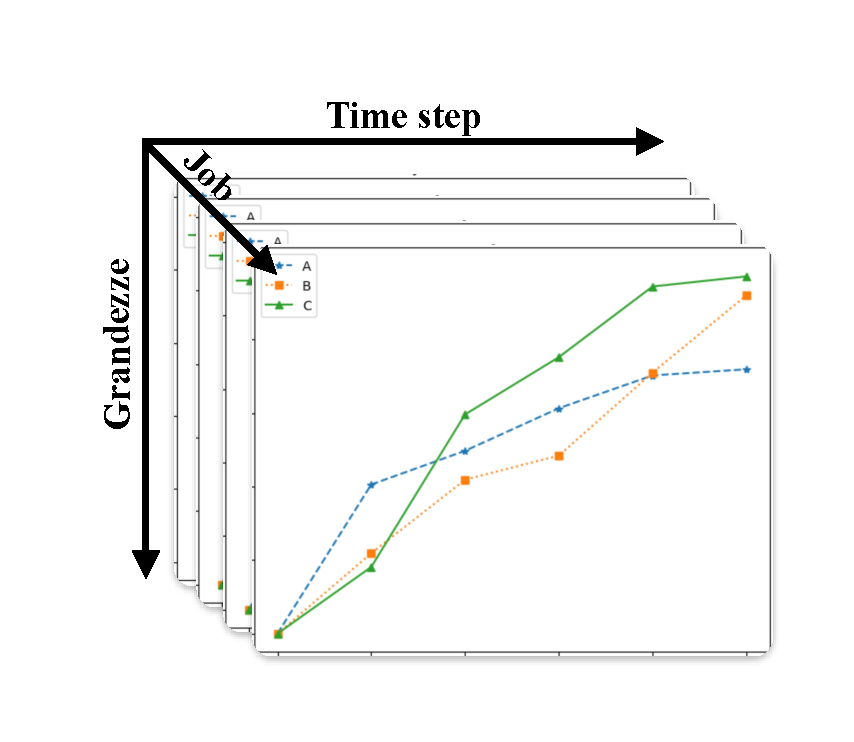
\includegraphics[trim=0cm 1.5cm 0cm 1.5cm, clip, width=0.5\linewidth]{multiple_multivariate_time-series}
   \caption{Rappresentazione tridimensionale delle multiple serie storiche
   multivariate}
   \label{fig:multiple_multivariate_time-series}
\end{figure}

Per gestire serie di dati con lunghezze diverse, possiamo utilizzare due
strategie: lo zero-padding e il troncamento. Lo zero-padding si applica alle
sequenze più corte, aggiungendo zeri fino a raggiungere una lunghezza
prefissata. Invece, il troncamento si usa per ridurre le sequenze più lunghe,
tagliandole fino a che non raggiungono la stessa lunghezza prestabilita. La
classe \texttt{Preprocessor} implementa entrambe le tecniche: stabilisce una
lunghezza fissa per tutte le sequenze, troncando quelle che eccedono questa
lunghezza e applicando lo zero-padding a quelle che non la raggiungono.

Una volta ottenute serie storiche di uguale lunghezza, vengono applicate le
seguenti trasformazioni, in base al modello utilizzato:

\begin{itemize}
    \item \textbf{Trasformazione in colonne}: Ogni elemento di ogni lista diventa una colonna
        separata nel dataset. Ad esempio, con un sottocampionamento a 15
        minuti per un giorno, avremo 96 time step, corrispondenti a 96 colonne
        per ciascuna serie temporale.
    \item \textbf{Trasformazione in righe}: 
        Gli elementi nelle stesse posizioni nelle liste formano righe
        distinte. Quindi, con un sottocampionamento a 15 minuti per un giorno,
        otteniamo 96 righe per ogni job.
\end{itemize}

\subsection{Creazione delle feature}

Dopo aver convertito le serie storiche in formato numerico, rimangono alcune
colonne, come \texttt{job} e \texttt{queue}, che sono di tipo categorico
nominale e che necessitano anch'esse di essere convertite in formato numerico.
Inoltre, è importante assicurarsi che le colonne numeriche siano sulla stessa
scala, poiché le differenze di scala possono portare a prestazioni subottimali
nei modelli. Quindi, un passo importante nella preparazione dei dati è il
ridimensionamento di queste colonne.

\paragraph{One-hot encoding.} 

Una possibile soluzione per gestire le colonne di tipo categorico potrebbe
essere quella di assegnare un valore intero a ciascun valore categorico.
Tuttavia, questa strategia può indurre il modello a interpretare i valori
numerici vicini come simili e quelli distanti come dissimili, il che non è
appropriato per le colonne di tipo categorico nominale.

Per risolvere questo problema, si può utilizzare la tecnica dell'one-hot
encoding, che crea una colonna binaria per ogni valore categorico: la colonna
sarà impostata a 1 per la categoria corrispondente e a 0 per tutte le altre.
Sfortunatamente, il one-hot encoding può generare un eccessivo numero di
colonne in presenza di colonne con alta cardinalità, come \texttt{job}
($\mathcal{O}(\text{numero righe})$) o \texttt{queue} ($\mathcal{O}(50)$). In
questi casi, si rischia di avere troppe feature irrilevanti, compromettendo
l'efficacia del modello di Machine Learning. 

Per garantire che il modello impari efficacemente dai dati, è fondamentale
selezionare feature rilevanti ed eliminare quelle irrilevanti. È altresì
importante che il modello interpreti i dati in modo simile a come li
percepiamo noi, evidenziando le caratteristiche salienti dei dati e la
struttura del problema. 

Per far ciò, sono state create due nuove colonne, \texttt{job type} e
\texttt{job work type} (vedi figura ~\ref{fig:job_type_and_job_work_type}),
seguite dall'applicazione dell'one-hot encoding. La prima colonna raggruppa i
gruppi di utenti, in LHC e non-LHC, che, come osservato nell'analisi
preliminare, hanno meccanismi interni diversi e potrebbero comportarsi in
maniera differente. Allo stesso modo, viene estratto il \verb|submit_node|
dalla colonna \texttt{job}, dove ogni ID è composto da
\verb|jobid.idx_submitnode|, e classificato i job in base al fatto che il
\verb|submit_node| sia ``sn0x'' o ``ce0x'', distinguendo così i job sottomessi
dagli utenti interni del CNAF da quelli degli utenti esterni.

\begin{figure}[!ht]
    \centering
    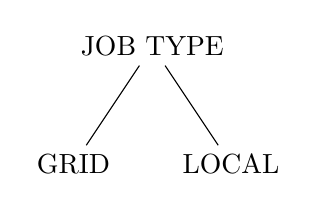
\begin{tikzpicture}[sibling distance=2cm]
        \node {JOB TYPE}
        child {node {GRID}}
        child {node {LOCAL}};
    \end{tikzpicture}
    \hspace{2cm}
    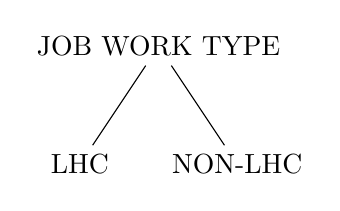
\begin{tikzpicture}[sibling distance=2cm]
        \node {JOB WORK TYPE}
        child {node {LHC}}
        child {node {NON-LHC}};
    \end{tikzpicture}
    \caption{Visualizzazione delle nuove colonne \texttt{job type} e \texttt{job work type}}
    \label{fig:job_type_and_job_work_type}
\end{figure}

\paragraph{Ridimensionamento delle feature.}

La normalizzazione è il processo che ridimensiona i dati in un range tra 0 e
1. La formula è $X'=\frac{(X-X_{min})}{X_{max}-X_{min}}$, dove $X_{min}$ e
$X_{max}$ sono rispettivamente i valori minimi e massimi della feature. La
standardizzazione trasforma i dati in modo che abbiano media 0 e varianza di
1. La formula è $X'=\frac{X-\mu}{\sigma}$.

Ridimensionare i dati è 

Ridimensionare i dati è importante perché aiuta i modelli a convergere meglio
ai parametri migliori

%Scaling is important because it preconditions the data to facilitate
%optimization. Putting the features on the same scale stretches the
%optimization surface to ameliorate narrow valleys, because these valleys make
%optimization very challenging, especially optimization using gradient descent
% . The reason we scale data is to improve gradient descent dynamics,

%Which scaling method works best depends on the problem,because different
%problems have different optimization surfaces.
% A very general strategy is to carry out an experiment: test how well the
% model works with alternative methods 
%
%Lecun
% the network training converges faster if its inputs are whitened – i.e.,
% linearly transformed to have zero means and unit variances

%For instance many elements used in the objective function of a learning
%algorithm (such as the RBF kernel of Support Vector Machines or the L1 and L2
%regularizers of linear models) assume that all features are centered around 0
%and have variance in the same order.

%http://yann.lecun.com/exdb/publis/pdf/lecun-98b.pdf
%sklearn

%d the algorithm, ad esempio gli alberi decisionali, does not make assumptions
%about the distribution. It is a good technique when we did not know about the
%distribution of data or when we know the distribution is not gaussian.

%doesn't reduce the effect of outliers, ma li scala them down into a fixed
%range, where the largest occuring data point corresponds to the maximum value
%and the smallest one corresponds to the minimun value.
%
%Normalization is a good technique to use when you do not know the distribution
%of your data or when you know the distribution is not Gaussian (a bell curve).
%
%Standardization presupposes that the distribution of your data is Gaussian
%
%La normalizzazione è cruciale per modelli come le reti neurali.

\subsection{Etichettatura dei dati}

In base alla presenza di etichette nei dati, possiamo distinguere tra
apprendimento supervisionato e non supervisionato. Nell'apprendimento
supervisionato, i modelli vengono addestrati con un dataset, dove ogni esempio
è associato a un'etichetta, rappresentante un valore categorico o numerico.
Durante l'addestramento, il modello tenta di prevedere le etichette per esempi
che non ha mai visto prima. Le predizioni sono poi confrontate con le
etichette per calcolare l'errore, che indica quanto le predizioni del modello
si discostano dai valori reali. L'obiettivo è migliorare la precisione del
modello minimizzando l'errore, tipicamente attraverso la discesa del
gradiente.

Attualmente, il dataset non include etichette che identifichino quali job
siano zombie, il che ci impedisce di impostare un apprendimento
supervisionato. Per generare le etichette, calcoliamo il tempo di esecuzione
di ogni job come \verb|int((maxt - mint) / 86400)| per ottenere il numero
di giorni di esecuzione. Poi, con la colonna \texttt{job\_type}, etichettiamo
come job zombie quelli che soddisfano la condizione:

\begin{verbatim}
    se giorni > (3 se job_type == `grid', altrimenti 7) e fail == 1 
\end{verbatim}

\subsection{Tecniche di bilanciamento dei dati}

Nella sezione~\ref{sec:job_analysis}, abbiamo osservato che i job zombie sono
estremamente più rari dei job normali, con un rapporto di 1 a 10,000. A causa
di questo forte sbilanciamento, il classificatore potrebbe semplicemente
apprendere a identificare tutti gli esempi come job normali (etichettati come
0), ottenendo così un errore apparentemente molto basso, ma in realtà
ignorando completamente i job zombie, che sono esattamente quelli che
desideriamo identificare. 

Per tentare di ridurre il bias del modello verso la classe maggioritaria sono
state adottate tre tecniche in combinazione: sottocampionamento,
sovracampionamento e Cost-sensitive learning. Queste tecniche mirano a
bilanciare la distribuzione delle classi nel dataset e a migliorare la
capacità del modello di distinguere tra job normali e job zombie. 

\paragraph{Sottocampionamento casuale.} Il sottocampionamento casuale è una
strategia molto semplice in cui vengono cancellati casualmente degli esempi di
job normali dal dataset. Tuttavia, ciò può comportare la perdita di
informazioni preziose per il modello, causando una perdita della sua
precisione \cite{he2013}.

\paragraph{Sovracampionamento.}
\label{par:vae}

Un'alternativa è il sovracampionamento dei job zombie. Il metodo più semplice
consiste nell'aggiungere duplicati di esempi già presenti nel dataset;
tuttavia, ciò non fornisce nuove informazioni utili al modello. Un approccio
più efficace è la generazioni di nuovi esempi artificiali, che sono varianti
dei job zombie \cite{brownlee2021}. 

Pertanto, si è scelto di usare una variante dell'autoencoder, nota come
\textbf{variational autoencoder} \cite{kingma2022}, per generare varianti di
job zombie a partire dai job zombie dell'intero 2021. Gli autoencoder
tradizionali apprendono funzioni per mappare esempi in punti nello spazio
latente e viceversa, per mappare le loro rappresentazioni compresse dallo
spazio latente allo spazio originale. Tuttavia, se si prende una variante di
un esempio nello spazio latente, il decoder $g(h)$ genererà un output privo di
senso, in quanto non è in grado di gestire regioni dello spazio mai esplorate.
Il variational autoencoder risolve questo problema facendo sì che l'encoder
anziché restituire una rappresentazione compressa $h$, fornisca una media
$\mu$ e una deviazione standard $\sigma$. Intuitivamente, la rappresentazione
compressa viene campionata da una distribuzione gaussiana caratterizzata dalla
media $\mu$ e dalla deviazione standard $\sigma$. In questo modo, il decoder
impara a mappare non solo un singolo punto nello spazio latente, ma anche
tutti i punti nelle sue vicinanze (vedi figura~\ref{fig:vae_comparison})
\cite{shafkat2018}.

Tuttavia, il sovracampionamento aumenta il rischio di overfitting, cioè la
possibilità che il modello si adatti eccessivamente ai dati di addestramento,
perdendo così la capacità di generalizzare su dati nuovi\cite{fernandez2018}.

\begin{figure}
    \centering
    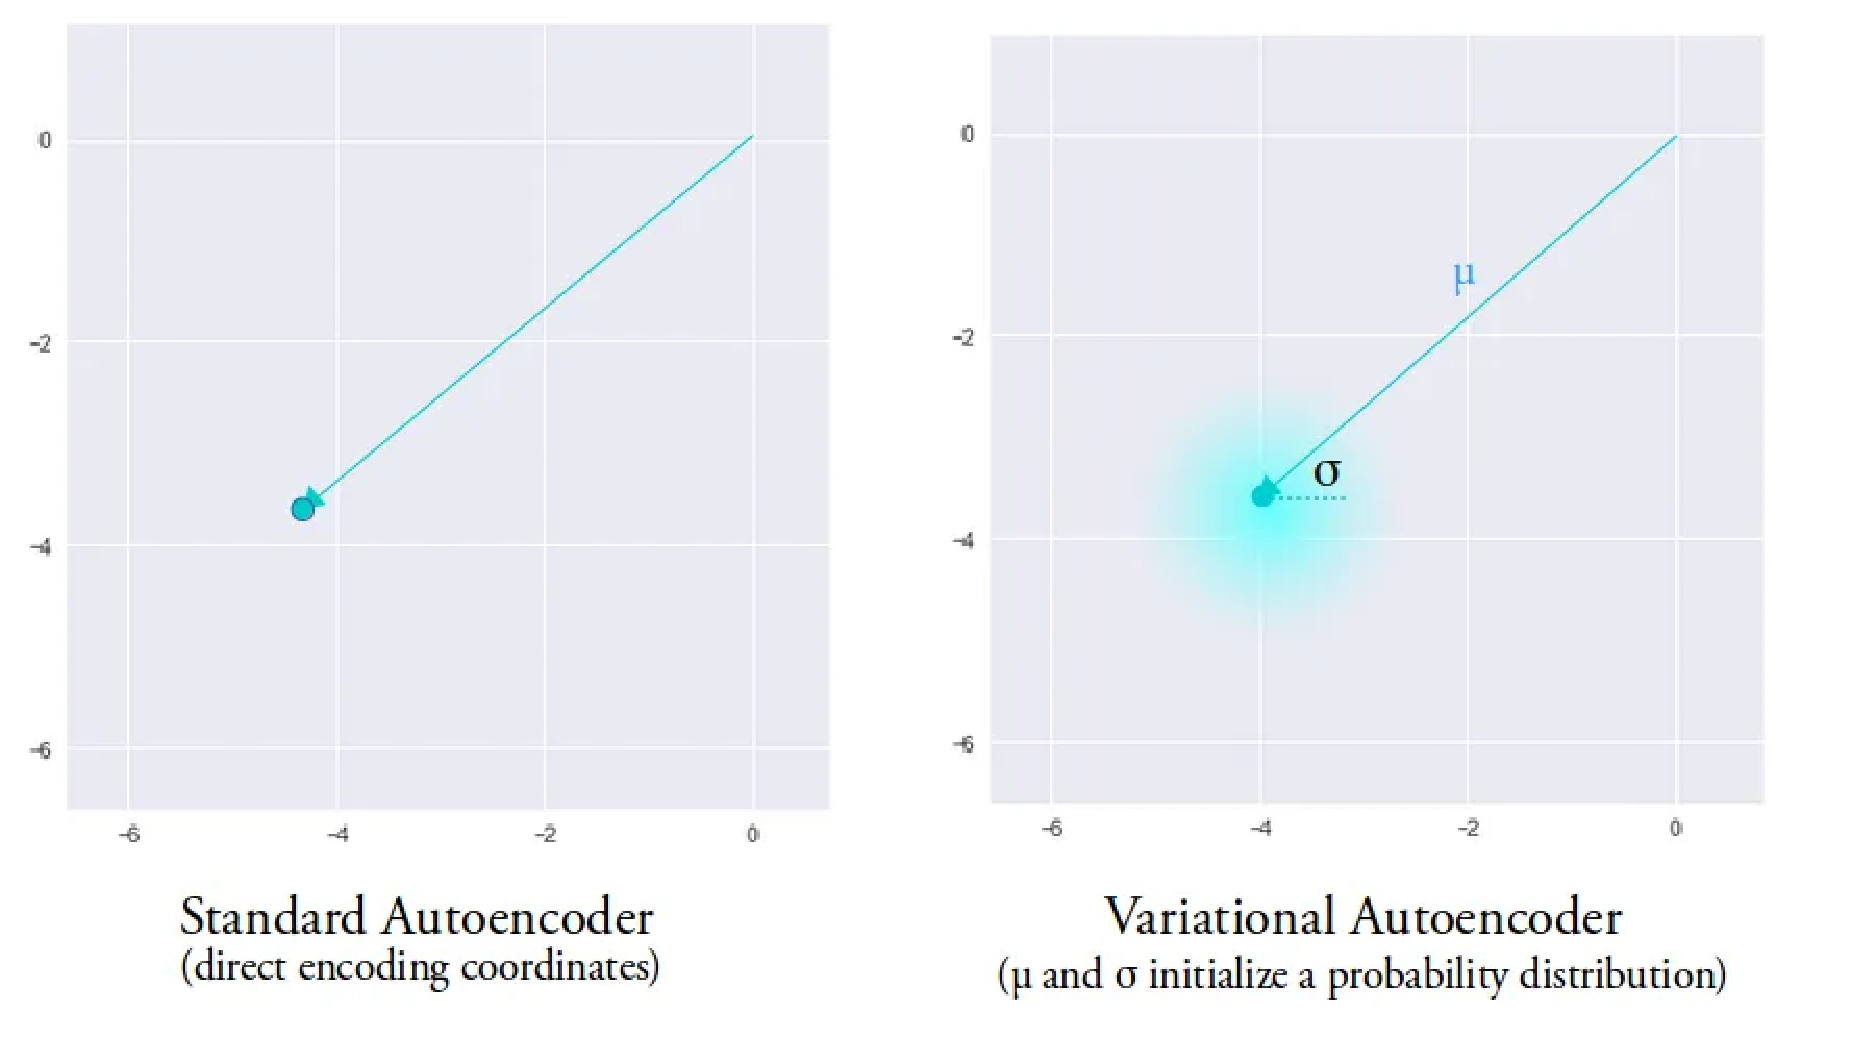
\includegraphics[width=0.95\linewidth]{vae_comparison}
    \caption{Rappresentazioni compresse in un autoencoder tradizionale e un
    variational autoencoder \cite{shafkat2018}}
    \label{fig:vae_comparison}
\end{figure}

\paragraph{Cost-sensitive learning.}

Possiamo distinguere gli errori commessi dal modello in falsi positivi e falsi
negativi in base a due criteri: un errore è falso positivo quando il modello
identifica erroneamente un job come zombie nonostante non lo sia; è invece un
falso negativo quando il modello etichetta come normale un job che in realtà è
zombie.

Assegnando un valore diverso, che definiamo ``costo'', ai falsi positivi e ai
falsi negativi, e minimizzando il costo totale\footnote{$\text{Costo totale} =
    C_{FN} \cdot
FN + C_{FP} \cdot FP$} derivante dalle predizioni
errate, il modello imparerà durante l'addestramento ad attribuire diversa
importanza ai vari tipi di errori.


\section{Selezioni dei modelli}

% anomaly detection vs classification

Anomaly detection is not binary classification because our models do not
explicitly model an anomaly. Instead, they learn to recognize only what it is
to be normal. In fact, we could use binary classification if we had a lot of
anomalies of all kinds to work with… But then, they wouldn’t be anomalies
after all!

\subsection{Classificazione}

\subsubsection{XGBoost}

\subsubsection{Deep learning}

% Representation of instances must be appropriate
%Most ML models requires item as a real-valued vector (x1, x2, ...)
%Each value of a vector encodes a specific feature
%Features must be carefully chosen in order to obtain effective models
%Feature engineering can be a cumbersome task

% at each iteration, equation requires a complete pass through the intere
% dataset in orde to compute the gradient. 

% batch learning an entire batch of data must be considered before weight are
% updated

%L'input è rappresentato da un tensore 3D (batch size, time steps,
%features)
%To train the LSTM you use the typical Mini-batch training. Make sure
%you don't propagate the state for batch sample 𝑖 to sample 𝑖+1 in
%order to treat them individually (in Keras you set the stateful flag
%to False)
% Essentially, the author is describing a means for forecasting sales
% with LSTM whereby the model is trained on a mini-batch (or subset) of
% one series, and then a new series is selected.

%This would have the advantage of essentially creating a unified series
%that takes the characteristics of all weather stations into account -
%which allows for maximum utilisation of the data, as well as allowing
%the network to learn patterns from all stations - not just one or a
%select few.
%An RNN (or a Transformer) could use any of/all of the history that you
%give it. But that's assuming that the history is useful for the
%predictions you're making.

\subsection{Novelty detection}

%un altro modo di poter appocciare lo stesso problema di individuare i job
%zombie dai job normali è affrontando un task di novelty detection.
%
%In questo il task è 
%
%ricordiamo che un autoencoder è addestrato per ridurre al minimo l'errore di
%ricostruzione
%
%“new and not resembling something formerly known or
%used”.
%
%in più permette explainability
%
%is assumed to be trained on a clean dataset, uncontaminated by outliers
%
%come abbiamo parlato nel paragrafo ~\ref{par:vae} gli input che durante
%l'addestramento dell'autoencoder non sono mai stati visti il decoder non saprà
%ricostruirlo correttamente e in questo caso darà un errore di ricostruzione
%molto alto $\epsilon=\lVert x-g(f(x))\rVert_2$. 
%
%In questo caso per determinare se un dato esempio è normale o zombie, ci
%basiamo sull'errore di ricostruzione e guardiamo nuovamente le etichette.
%
%effettuiamo l'addestramento su un dataset clean e poi su un altro dataset in
%un periodo successivo andiamo a settare un threshold sull'errore di
%ricostruzione in base al quale, quelli che sono sopra al threshold sono job
%zombie (1) e quelli che sono sotto job normali (0). Come al solito andiamo a
%minimizzare su questo nuovo dataset l'errore o il costo cercando di.
%
%The test sample x is more likely to be novel as the error ε(x) becomes larger,
%because it means that x is farther from the manifold that the autoencoder
%describes.

% ovviamente l'encoder e il decoder che abbiamo descritto come delle funzioni,
% nella realtà sono architetture di reti neurali, e possono essere realizzate
% per poter definire un funzione non lineare

\begin{figure}[!ht]
    \centering
    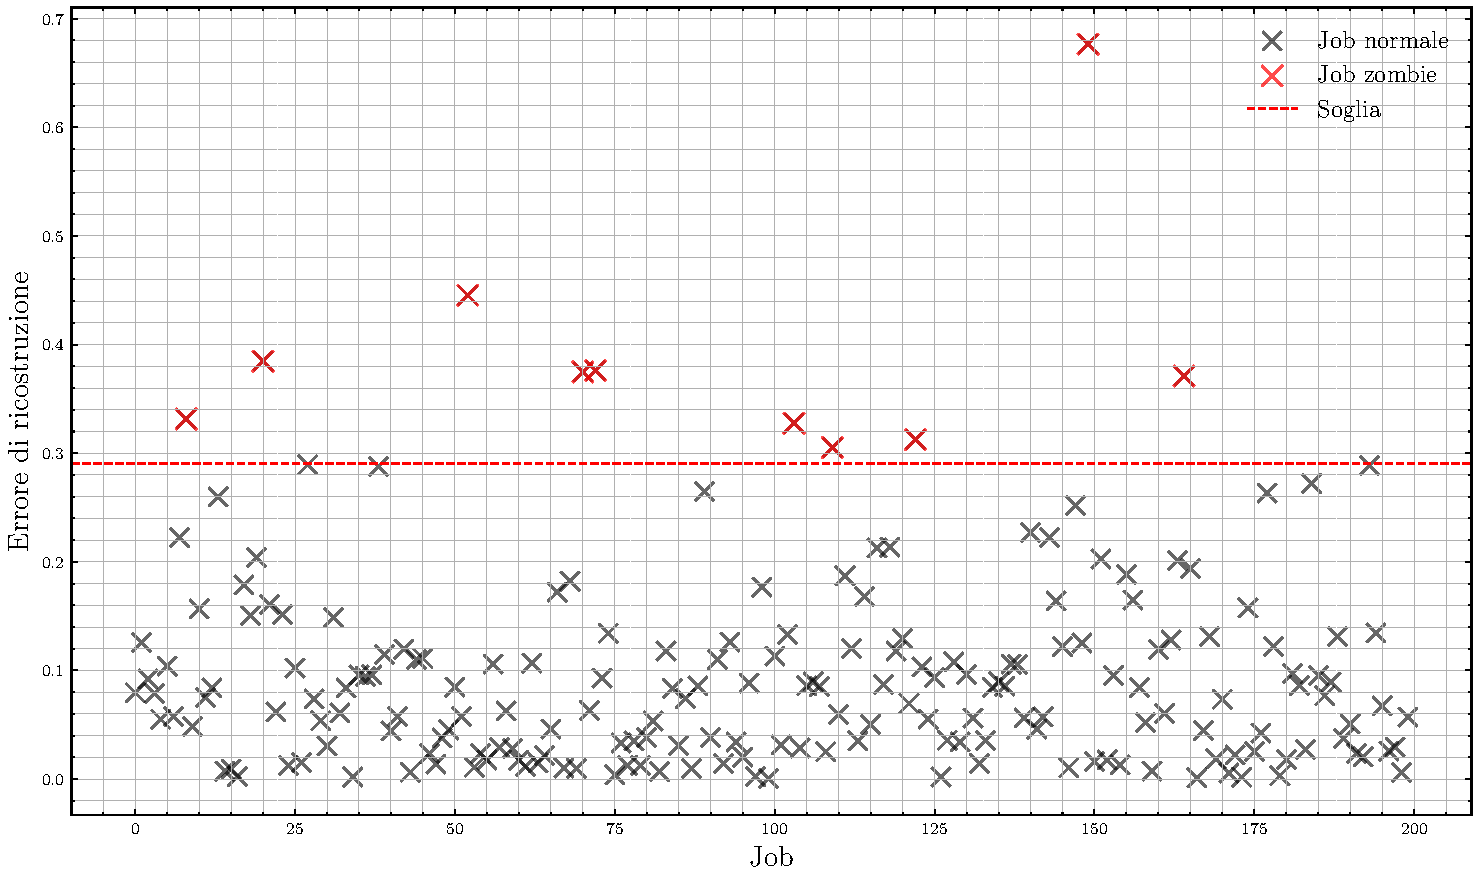
\includegraphics[width=0.95\linewidth]{reconstruction_error}
    \caption{}
    \label{fig:reconstruction_error}
\end{figure}
